\chapter{Planification et Estimation}

\section{Découpage du Projet en Sprints}

Nous avons utilisé une méthode itérative pour planifier le projet, en le découpant en \textbf{quatre Sprints} (incluant un Sprint 0 de cadrage).

\subsection{Sprint 0 : Cadrage (01/04 --- 02/04/2026)}

\begin{table}[H]
\centering
\begin{tabularx}{\textwidth}{X L{5cm} C{2cm}}
\toprule
\textbf{\color{primarycolor}Tâche} &
\textbf{\color{primarycolor}Livrable} &
\textbf{\color{primarycolor}Statut} \\
\midrule
Cadrage du besoin métier (MOA) & Cahier des charges informel & Fait \\
Choix de l'architecture (Kappa vs Lambda) & Document de décision & Fait \\
Mise en place de Taiga (Kanban) & Board configuré & Fait \\
Planification (Gantt) & Diagramme de Gantt & Fait \\
\bottomrule
\end{tabularx}
\caption{Sprint 0 --- Cadrage du projet}
\end{table}

\subsection{Sprint 1 : Infrastructure (06/04 --- 08/04/2026)}

\begin{table}[H]
\centering
\begin{tabularx}{\textwidth}{X L{5cm} C{2cm}}
\toprule
\textbf{\color{primarycolor}Tâche} &
\textbf{\color{primarycolor}Livrable} &
\textbf{\color{primarycolor}Statut} \\
\midrule
Rédiger le \texttt{docker-compose.yml} & Fichier de configuration & Fait \\
Lancer Zookeeper + Kafka & Conteneurs opérationnels & Fait \\
Lancer Flink (JobManager + TaskManager) & Interface Flink accessible & Fait \\
Créer le topic \texttt{clics\_ecommerce} & Topic Kafka fonctionnel & Fait \\
Test : produire/consommer un message & Preuve de fonctionnement & Fait \\
\bottomrule
\end{tabularx}
\caption{Sprint 1 --- Mise en place de l'infrastructure}
\end{table}

\subsection{Sprint 2 : Simulateur et Topologies (09/04 --- 13/04/2026)}

\begin{table}[H]
\centering
\begin{tabularx}{\textwidth}{X L{5cm} C{2cm}}
\toprule
\textbf{\color{primarycolor}Tâche} &
\textbf{\color{primarycolor}Livrable} &
\textbf{\color{primarycolor}Statut} \\
\midrule
Développer \texttt{simulateur.py} (v1) & Script de simulation basique & Fait \\
Améliorer \texttt{simulateur.py} (v2 : bots, prix, sessions) & Simulateur complet & Fait \\
Développer la topologie de filtrage & \texttt{filtrage.py} fonctionnel & Fait \\
Développer la topologie d'agrégation & \texttt{agregation.py} fonctionnel & Fait \\
Développer la détection d'abandon & \texttt{detection\_abandon.py} fonctionnel & Fait \\
Configurer les topics avec rétention & \texttt{setup\_topics.sh} & Fait \\
\bottomrule
\end{tabularx}
\caption{Sprint 2 --- Développement du simulateur et des topologies}
\end{table}

\subsection{Sprint 3 : Validation et Rapport (14/04 --- 16/04/2026)}

\begin{table}[H]
\centering
\begin{tabularx}{\textwidth}{X L{5cm} C{2cm}}
\toprule
\textbf{\color{primarycolor}Tâche} &
\textbf{\color{primarycolor}Livrable} &
\textbf{\color{primarycolor}Statut} \\
\midrule
Test de replay & \texttt{test\_replay.py} & Fait \\
Validation de cohérence & Résultats documentés & Fait \\
Rédaction du rapport final & Rapport complet & Fait \\
Préparation de la présentation & Slides & Fait \\
\bottomrule
\end{tabularx}
\caption{Sprint 3 --- Validation et documentation}
\end{table}

\section{Le Diagramme de Gantt}

Le suivi temporel a été modélisé à l'aide de \textbf{GanttProject}. Cet outil nous a permis d'ordonnancer les tâches, de visualiser les dépendances et d'identifier le \textbf{chemin critique} du projet.

\begin{borderedfigure}
    \centering
    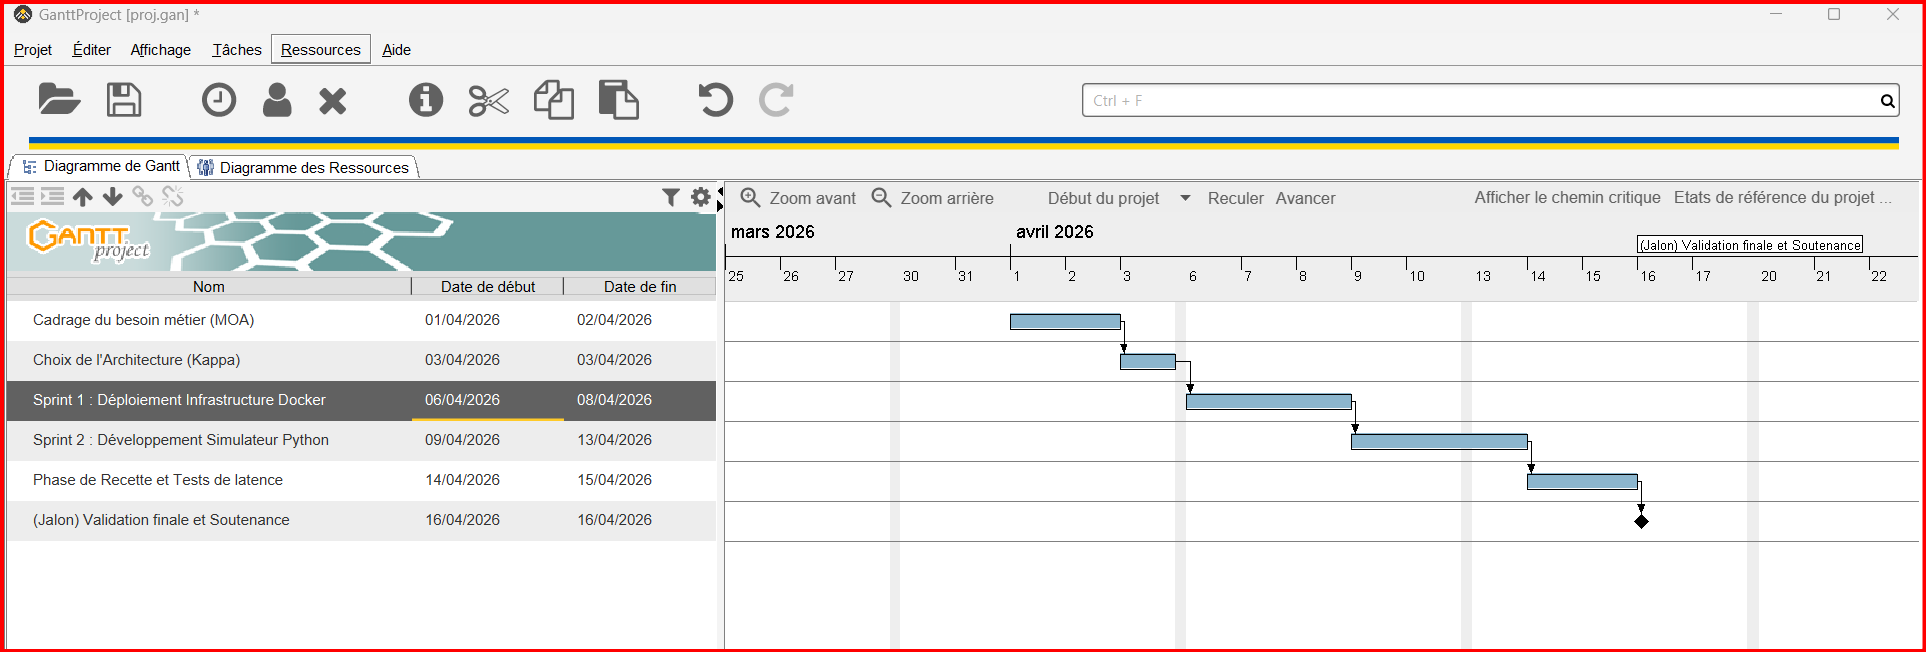
\includegraphics[width=\textwidth]{../screenshots/Gantt.png}
    \captionof{figure}{Diagramme de Gantt du projet --- planification sur 3 semaines}
\end{borderedfigure}

\section{User Stories}

Les fonctionnalités ont été exprimées sous forme de \textbf{User Stories}, priorisées et affectées aux sprints :

\begin{table}[H]
\centering
\begin{tabularx}{\textwidth}{C{1cm} X C{1.5cm} C{1.5cm}}
\toprule
\textbf{\color{primarycolor}\#} &
\textbf{\color{primarycolor}User Story} &
\textbf{\color{primarycolor}Priorité} &
\textbf{\color{primarycolor}Sprint} \\
\midrule
US1 & En tant que MOE, je veux déployer Kafka pour recevoir les événements & Haute & Sprint 1 \\
\addlinespace[0.1cm]
US2 & En tant que MOE, je veux un simulateur pour générer des données test & Haute & Sprint 2 \\
\addlinespace[0.1cm]
US3 & En tant que MOA, je veux filtrer les bots pour avoir des stats fiables & Haute & Sprint 2 \\
\addlinespace[0.1cm]
US4 & En tant que MOA, je veux voir les stats par produit en temps réel & Haute & Sprint 2 \\
\addlinespace[0.1cm]
US5 & En tant que MOA, je veux être alerté des abandons de panier & Haute & Sprint 2 \\
\addlinespace[0.1cm]
US6 & En tant que MOE, je veux valider la cohérence par replay & Moyenne & Sprint 3 \\
\bottomrule
\end{tabularx}
\caption{Backlog des User Stories}
\end{table}

\section{Estimation des Charges (Planning Poker)}

Pour éviter de sous-estimer le temps de développement --- risque fréquent identifié dans le Chapitre 8 du cours ---, nous avons utilisé la méthode du \textbf{Planning Poker}. Cette approche collaborative a permis d'estimer les User Stories de manière consensuelle.

\begin{table}[H]
\centering
\begin{tabularx}{\textwidth}{X C{2.5cm} C{2.5cm} C{2cm}}
\toprule
\textbf{\color{primarycolor}User Story} &
\textbf{\color{primarycolor}Estimation initiale} &
\textbf{\color{primarycolor}Consensus} &
\textbf{\color{primarycolor}Réel} \\
\midrule
US1 : Déployer Kafka & 3 & 5 & 5 \\
US2 : Simulateur & 2 & 3 & 3 \\
US3 : Filtrage & 3 & 3 & 3 \\
US4 : Agrégation & 5 & 5 & 5 \\
US5 : Détection abandon & 5 & 8 & 5 \\
US6 : Replay & 3 & 3 & 3 \\
\bottomrule
\end{tabularx}
\caption{Résultats du Planning Poker --- estimation en story points}
\end{table}

\begin{infobox}
    \textbf{Leçon apprise :} L'estimation initiale sous-estimait souvent la complexité des tâches. Le Planning Poker permet d'avoir des estimations plus réalistes grâce au consensus de l'équipe et à la prise en compte de l'incertitude technique.
\end{infobox}

\section{Vélocité de l'Équipe}

La vélocité mesure la capacité de production de l'équipe en story points par sprint :

\begin{table}[H]
\centering
\begin{tabularx}{\textwidth}{L{3cm} C{3cm} C{3cm} C{3cm}}
\toprule
\textbf{\color{primarycolor}Sprint} &
\textbf{\color{primarycolor}Points prévus} &
\textbf{\color{primarycolor}Points réalisés} &
\textbf{\color{primarycolor}Vélocité} \\
\midrule
Sprint 1 & 8 & 8 & 100\% \\
Sprint 2 & 13 & 13 & 100\% \\
Sprint 3 & 8 & 8 & 100\% \\
\midrule
\textbf{Total} & \textbf{29} & \textbf{29} & \textbf{100\%} \\
\bottomrule
\end{tabularx}
\caption{Vélocité de l'équipe par sprint}
\end{table}
